\chapter{Antennen}
 \section{Grundbegriffe und Elementardipole}
 \subsection{Hertzscher Dipol}
	  \begin{center}
		  \tdplotsetmaincoords{60}{110}

%define polar coordinates for some vector
%TODO: look into using 3d spherical coordinate system
\pgfmathsetmacro{\rvec}{.5}
\pgfmathsetmacro{\thetavec}{30}
\pgfmathsetmacro{\phivec}{60}

%start tikz picture, and use the tdplot_main_coords style to implement the display 
%coordinate transformation provided by 3dplot
\begin{tikzpicture}[scale=5,tdplot_main_coords]

	%set up some coordinates 
	%-----------------------
	\coordinate (O) at (0,0,0);

	%determine a coordinate (P) using (r,\theta,\phi) coordinates.  This command
	%also determines (Pxy), (Pxz), and (Pyz): the xy-, xz-, and yz-projections
	%of the point (P).
	%syntax: \tdplotsetcoord{Coordinate name without parentheses}{r}{\theta}{\phi}
	\tdplotsetcoord{P}{\rvec}{\thetavec}{\phivec}

	%draw figure contents
	%--------------------

	%draw the main coordinate system axes
	\draw[thick,->] (0,0,0) -- (.5,0,0) node[anchor=north east]{$x$};
	\draw[thick,->] (0,0,0) -- (0,.5,0) node[anchor=north west]{$y$};
	\draw[thick,->] (0,0,0) -- (0,0,.5) node[anchor=south,pos=0.95]{$z$};

	%draw a vector from origin to point (P) 
	\draw[-stealth,color=red,thick] (O) -- (P) node[midway, below]{$\vec{r} $};
	\draw[-stealth,color=green,thick] (P) -- +(0,0,0.2) node[above]{$ \vec{\ubar{A}}= \ubar{A}_z\vu{z}$};

	%draw projection on xy plane, and a connecting line
	\draw[dashed, color=red] (O) -- (Pxy);
	\draw[dashed, color=red] (P) -- (Pxy);

	%draw the angle \phi, and label it
	%syntax: \tdplotdrawarc[coordinate frame, draw options]{center point}{r}{angle}{label options}{label}
	\tdplotdrawarc{(O)}{0.2}{0}{\phivec}{anchor=north}{$\varphi$}

	%set the rotated coordinate system so the x'-y' plane lies within the
	%"theta plane" of the main coordinate system
	%syntax: \tdplotsetthetaplanecoords{\phi}
	\tdplotsetthetaplanecoords{\phivec}

	%draw theta arc and label, using rotated coordinate system
	\tdplotdrawarc[tdplot_rotated_coords]{(0,0,0)}{0.3}{0}{\thetavec}{anchor=south west}{$\vartheta$}

	%draw some dashed arcs, demonstrating direct arc drawing
	%\draw[dashed,tdplot_rotated_coords] (\rvec,0,0) arc (0:90:\rvec);
	%\draw[dashed] (\rvec,0,0) arc (0:90:\rvec);

	%set the rotated coordinate definition within display using a translation
	%coordinate and Euler angles in the "z(\alpha)y(\beta)z(\gamma)" euler rotation convention
	%syntax: \tdplotsetrotatedcoords{\alpha}{\beta}{\gamma}
	\tdplotsetrotatedcoords{\phivec}{\thetavec}{0}

	%translate the rotated coordinate system
	%syntax: \tdplotsetrotatedcoordsorigin{point}
	\tdplotsetrotatedcoordsorigin{(P)}

	%use the tdplot_rotated_coords style to work in the rotated, translated coordinate frame
	\draw[thin,tdplot_rotated_coords,->] (0,0,0) -- (.1,0,0) node[anchor=north west]{$\vu{\vartheta}$};
	\draw[thin,tdplot_rotated_coords,->] (0,0,0) -- (0,.1,0) node[anchor=west]{$\vu{\varphi}$};
	\draw[thin,tdplot_rotated_coords,->] (0,0,0) -- (0,0,.1) node[anchor=south]{$\vu{r}$};

	\node (a) [cylinder, shape border rotate=90, draw, minimum height=5mm, minimum width=2mm,yshift=-1mm] {};
	\draw [<->] ([xshift=-2pt]a.before bottom) -- ([xshift=-2pt]a.after top) node [midway, left] {$\ell$};

\end{tikzpicture}
	  \end{center}
		  Der \textbf{Hertzsche Dipol} ist eine wichtige Idealisierung einer lokalen Quelle von elektromagnetischen Wellen. Hertzsche Dipole werden auch in der Modellierung von Antennen und als Bezugsgröße für Antennencharakteristiken genutzt, sie sind \textbf{Elementardipole}. Realisiert wird der Hertzsche Dipol durch einen sehr kurzen geraden Leiter, auf dem ein Wechselstrom (in der Regel harmonisch) eingeprägt ist. Von einem \textbf{Hertzschem Dipol} spricht man, wenn
		  \begin{enumerate}
		  	\item Die Länge \(\ell\) des Leiters \textbf{wesentlich kleiner als die Wellenlänge} \(\lambda\) ist: \(\ell \ll \lambda\).
		  	\item Der Leiter ist \textbf{linienförmig}.
		  	\item Die Stromverteilung auf dem Leiter ist \textbf{konstant}: \(\underline{I}(\vec{r}^\prime ) = \underline{I} \)
		  \end{enumerate}
		  Der ideale Hertzsche Dipol kann durch extrem kurze Antennen (\(\ell < \frac{\lambda}{10}\)) tatsächlich \textbf{näherungsweise} realisiert werden.
		  \subsection{Potential und Felder für den Hertzschen Dipol}
		  \subsubsection{Vektorpotential}
		  Für harmonische Zeitabhängigkeit gilt für das Vektorpotential in Lorenzeichung ($\nearrow$\ref{vekpotlor}$\Rightarrow$\ref{kompvekpot}):
		        \begin{equation}\label{vekpotdip}
			        \vec{\ubar{A}}(\vec{r} ) = \frac{\mu}{4\pi} \iiint\limits_V \frac{ \mathrm{e}^{-\mathrm{j} k|\vec{r} -\vec{r}^\prime |}}{|\vec{r} -\vec{r}^\prime |} \ubar{\vec{J}}(\vec{r}^\prime ) \dd^3  r\prime
		        \end{equation}
		   Mit einem \textbf{dünnen Leiter} in \(z\)-Richtung gilt \(\ubar{\vec{J}}(\vec{r}^\prime ) \dd^3  r\prime = \underline{I}(\vec{r}^\prime )\vu{z}\dd z^\prime \) und es folgt:
		        \begin{equation}
			        \vec{\ubar{A}}(\vec{r} ) = \frac{\mu}{4\pi} \int\limits_{-\frac{\ell}{2}}^{\frac{\ell}{2}} \frac{ \mathrm{e}^{-\mathrm{j} k |\vec{r} -\vec{r}^\prime |}}{|\vec{r} -\vec{r}^\prime |} \underline{I}(\vec{r}^\prime )\vu{z}\dd z^\prime
		        \end{equation}
		        Für einen \textbf{Dipol im Ursprung} (\(\vec{r}^\prime  \simeq \vec{0} \to |\vec{r} -\vec{r}^\prime | \simeq |\vec{r} |=r\)):
		        \begin{equation}
		        	\boxed{ \vec{\ubar{A}}(\vec{r} ) = \frac{\mu}{4\pi} \frac{ \mathrm{e}^{-\mathrm{j} kr}}{r} \underline{I}\vu{z}\int\limits_{-\frac{\ell}{2}}^{\frac{\ell}{2}} \dd z^\prime = \frac{\mu}{4\pi} \underline{I} \ell  \frac{ \mathrm{e}^{-\mathrm{j} kr}}{r} \vu{z}} =  \ubar{A}_z \vu{z}
		        \end{equation}
		        Für die folgende Rechnung ist es einfacher, das Vektorpotential in Kugelkoordinaten \((r,\vartheta,\varphi)\) zu schreiben:
		        \begin{align}
		        	\ubar{A}_r          & =   \ubar{A}_z  \cos\vartheta    &\implies & &    \Aboxed{ \ubar{A}_r & =  \frac{\mu}{4\pi} \underline{I} \ell  \frac{ \mathrm{e}^{-\mathrm{j} kr}}{r} \cos\vartheta}\\
		        	\ubar{A}_\vartheta &=  - \ubar{A}_z \sin\vartheta         &\implies&& \Aboxed{ \ubar{A}_\vartheta &=  - \frac{\mu}{4\pi} \underline{I} \ell  \frac{ \mathrm{e}^{-\mathrm{j} kr}}{r} \sin\vartheta} \\                                                         &&&&  \Aboxed{ \ubar{A}_\varphi &=0} 
		        \end{align}
		   \subsubsection{Magnetfeld}
			         Aus dem Vektorpotential berechnet sich unmittelbar das Magnetfeld (welches durch den Rotationsoperator nur eine $\varphi$-Komponente hat $\to$ Intuition: Strom in $z$-Richtung$\Rightarrow$ Magnetfeld mit $\varphi$-Komponente):
				              \begin{equation}\label{diphfeld}\begin{split}
						              \vec{\ubar{H}} &= \ubar{H}_\varphi \vu{\varphi} = \frac{1}{\mu} \rot  \vec{\ubar{A}} = \frac{1}{\mu} \frac{1}{r} \left[ \frac{\partial \left(r  \ubar{A}_\vartheta  \right)}{\partial r} - \frac{\partial  \ubar{A}_r}{\partial \vartheta} \right] \vu{\varphi} \\
						              &= \frac{1}{4\pi} \underline{I} \ell  \frac{ \mathrm{e}^{-\mathrm{j} kr}}{r}\sin\vartheta \left[\frac{1}{r} + \mathrm{j} k\right]\; \vu{\varphi}\\
						              &= \frac{1}{4\pi} \underline{I} \ell  \frac{ \mathrm{e}^{-\mathrm{j} kr}}{r^2} \sin\vartheta \left[1+\mathrm{j} k r \right]\; \vu{\varphi} \quad\quad\quad  |k = \frac{\omega}{ v_\mathrm{p}}\\
						              &= \frac{1}{4\pi} \frac{\omega^2}{ v_\mathrm{p}^2}\underline{I} \ell  \frac{ \mathrm{e}^{-\mathrm{j} kr}}{( kr)^2} \sin\vartheta \left[1+\mathrm{j} k r \right]\; \vu{\varphi} \\
						              \Aboxed{\vec{\ubar{H}}& = \left\{\frac{1}{4\pi} \frac{\omega^2}{ v_\mathrm{p}^2}\underline{I} \ell   \mathrm{e}^{-\mathrm{j} kr} \sin\vartheta \left[\frac{1}{( kr)^2}+ \frac{\mathrm{j}}{ k r} \right]\right\}\; \vu{\varphi}}
					              \end{split}\end{equation}
				        Wegen \( k r = 2\pi\frac{r}{\lambda}\) ist die Wellenlänge die \enquote{natürliche} Längeneinheit.
  \subsubsection{Elektrisches Feld}
	 Das Elektrische Feld könnte prinzipiell auch direkt aus dem Vektorpotential berechnet werden ($\nearrow$\ref{lorenzbdg}):
		        \begin{equation}\begin{split}
				        \div  \vec{\ubar{A}} + \mathrm{j}\omega \varepsilon\mu \ubar{\phi}  = 0 &\Rightarrow \ubar{\phi} = -\frac{1}{\mathrm{j}\omega \varepsilon\mu} \div  \vec{\ubar{A}}\\
				        \ubar{\vec{E}} = -\grad \ubar{\phi} - \mathrm{j}\omega  \vec{\ubar{A}} &\Rightarrow \ubar{\vec{E}}  = \frac{1}{\mathrm{j}\omega \varepsilon\mu} \grad \div  \vec{\ubar{A}}- \mathrm{j}\omega  \vec{\ubar{A}}
			        \end{split}\end{equation}
 Einfacher ist die Berechnung direkt über Maxwell-Gleichung ($\nearrow$\ref{durchf}), es wird genutzt, dass $ \ubar{\vec{J}} = \vec{0}$ im Lösungsgebiet gilt:
		        \begin{equation}
			        \rot \vec{\ubar{H}} = \ubar{\vec{J}} + \mathrm{j}\omega\varepsilon\ubar{\vec{E}} \Rightarrow \ubar{\vec{E}} = \frac{1}{\mathrm{j}\omega\varepsilon} \rot \vec{\ubar{H}}
		        \end{equation}
 Es ergibt sich:
		        \begin{equation}\label{dipefeld}\boxed{\begin{split}
				        \ubar{\vec{E}} = &\left\{\frac{1}{2\pi} Z \frac{\omega^2}{ v_\mathrm{p}^2}\underline{I} \ell   \mathrm{e}^{-\mathrm{j} kr} \cos\vartheta\left[\frac{1}{( kr)^2} - \frac{\mathrm{j}}{( kr)^3}\right]\right\} \vu{r} + \\
				        &\left\{ \frac{1}{4\pi} Z \frac{\omega^2}{ v_\mathrm{p}^2}\underline{I} \ell   \mathrm{e}^{-\mathrm{j} kr} \sin\vartheta\left[\frac{\mathrm{j}}{ kr}  + \frac{1}{( kr)^2} - \frac{\mathrm{j}}{( kr)^3} \right] \right\} \vu{\vartheta}
			        \end{split}}\end{equation}
		        Hierbei ist \(Z=\frac{|\ubar{\vec{E}}|}{|\vec{\ubar{H}}|} = \sqrt{\frac{\mu}{\varepsilon}} = \frac{ k}{\omega\varepsilon}\) der \textbf{Feldwellenwiderstand} ($\nearrow$\ref{feldwellenwid}).
  \subsection{Fernfeld und mittlere Energieflussdichte in großem Abstand zur Quelle}
Die allgemeine Feldlösung für den Hertzschen Dipol ist mit \ref{diphfeld} und \ref{dipefeld} gegeben. Sehr nah an der Quelle würden die Terme mit $(kr)^3$ dominieren (\textbf{Nahfeld}). Weit weg von der Quelle, dominiert der Term mit $(kr)$. Man spricht vom \textbf{Fernfeld}. Die \textbf{Grenze zum Fernfeld} ist bei kurzen Antennen durch die Bedingung \( k r \gg 1 \Rightarrow r \gg  \frac{\lambda}{2\pi} = \frac{ v_\mathrm{p}}{2\pi f}\) gegeben. Im Vakuum gelten die folgenden Werte:
\begin{center}
	\begin{tabular}{c||c|c|c|c|c}
		$f$                & $50\mathrm{Hz}$      & $1\mathrm{kHz}$   & $100\mathrm{MHz}$ & $1\mathrm{GHz}$  \\
		\hline
		$\frac{c}{2\pi f}$ & ${954.3}\mathrm{km}$ & $47.8\mathrm{km}$ & $0.48\mathrm{m}$  & $4.8\mathrm{cm}$
	\end{tabular}
\end{center}
Man erkennt, dass man erst bei hohen Frequenzen sinnvoll die Fernfeldnäherung anwenden kann. Im Fernfeld gilt für den Hertzschen Dipol:
		        \begin{align}
			        \Aboxed{\vec{\ubar{H}}= \ubar{H}_\varphi \; \vu{\varphi} =      & \frac{\mathrm{j}}{4\pi} \frac{\omega^2}{ v_\mathrm{p}^2}\underline{I} \ell  \frac{ \mathrm{e}^{-\mathrm{j} kr}}{ kr} \sin\vartheta \; \vu{\varphi}}                                             \\
			        \Aboxed{\ubar{\vec{E}} = \ubar{E}_\vartheta \; \vu{\vartheta} = & Z \frac{\mathrm{j}}{4\pi} \frac{\omega^2}{ v_\mathrm{p}^2}\underline{I} \ell  \frac{ \mathrm{e}^{-\mathrm{j} kr}}{ kr} \sin\vartheta\; \vu{\vartheta}} = Z\; \ubar{H}_\varphi \; \vu{\vartheta}
		        \end{align}
		   Es ist eine \href{https://www.didaktikonline.physik.uni-muenchen.de/programme/dipolstr/Dipolstr_leifi.html}{Animation} der Felder verfügbar.
	 Im Fernfeld berechnet sich die \textbf{mittlere Energieflussdichte} zu:
		        \begin{equation}\begin{split}
				        \vec{\ubar{S}} &= \frac{1}{2} \ubar{\vec{E}} \times \vec{\ubar{H}}^\star = \frac{1}{2} \left( Z \frac{\mathrm{j}}{4\pi} \frac{\omega^2}{ v_\mathrm{p}^2}\underline{I} \ell  \frac{ \mathrm{e}^{-\mathrm{j} kr}}{ kr} \sin\vartheta\; \vu{\vartheta} \right) \times \left(\frac{\mathrm{j}}{4\pi} \frac{\omega^2}{ v_\mathrm{p}^2}\underline{I} \ell  \frac{ \mathrm{e}^{-\mathrm{j} kr}}{ kr} \sin\vartheta \; \vu{\varphi} \right)^\star\\
				        &= \frac{1}{2} Z \left( \frac{1}{4\pi} \frac{\omega^2}{ v_\mathrm{p}^2}\frac{|\underline{I}| \ell}{ kr} \right)^2 \left(\sin\vartheta\right)^2 \; \vu{r}  \\
				        & = S_r(r,\vartheta) \; \vu{r} = \langle \vec{S} \rangle
			        \end{split}\end{equation}
		        Hervorzuheben ist die $\vu{r}$-Richtung des Energieflusses. Weiterhin gilt insbesondere $ \vec{\ubar{S}}\in\IR$, es gibt also einen reinen Wirkleistungsfluss. Außerdem ist $S\propto r^{-2}$, was intuitiv erscheint, da für die Kugeloberfläche $A=4\pi r^2$ gilt. Zudem ist die $\vartheta$-Abhängigkeit interessant. Grafisch ergibt sich folgender Verlauf:\\
		        \begin{minipage}{.5\textwidth}
	\centering
	\begin{tikzpicture}
		\draw[->] (-.1, 0) -- (pi+0.2, 0) node[right] {$\vartheta$};
		\draw[->] (0, -0.1) -- (0, 1.1) node[above] {$\sin^2\vartheta$};
		\draw[domain=0:pi, smooth, variable=\x, red, thick] plot ({\x}, {(sin(\x*180/pi))^2});
		\draw[thin] (0,0) -- (0,-0.1) node[below]{$0$};
		\draw[thin] (pi/2,0) -- (pi/2,-0.1) node[below]{$\frac{\pi}{2}$};
		\draw[thin] (pi,0) -- (pi,-0.1) node[below]{$\pi$};
	\end{tikzpicture}
\end{minipage}
\begin{minipage}{.5\textwidth}
	\centering
	\begin{tikzpicture}[scale=2]
		\draw[->] (-.1, 0) -- (1.2, 0) node[right] {$r$};
		\draw[->] (0, -0.6) -- (0, 0.6) node[above] {$z$};
		% \draw[thick,red] (0,0) \foreach \th in {1, ... ,180} { -- ({90-\th}:{(sin(\th))^2}) };
		\draw[thick,red,variable=\th,domain=0:180,samples=90]
		plot ( {(sin(\th))^3} , {cos(\th)*(sin(\th))^2} );
		\draw [thin] (0,0) -- (30:{(sin(60))^2}) node[midway, right]{$\sin^2\vartheta$};
		\draw [thin,-stealth] (0,0.4) arc (90:30:0.4) node[midway,above]{$\vartheta$};
	\end{tikzpicture}
\end{minipage}

  \subsection{Strahlungsdiagramm}
		   Das \textbf{Strahlungsdiagramm} ist die normierte Darstellung der mittleren Energieflussdichte (analog z.B. auch für Feldstärken definierbar), also von
		        \begin{equation}
			        \frac{S_r(r,\vartheta, \varphi)}{\max(S_r(r,\vartheta, \varphi))}.
		        \end{equation}
		   Dargestellt werden in der Regel die zweidimensionalen Hauptschnitte.
		   Für den Hertzschen Dipol ergeben sich das \textbf{\enquote{Horizontaldiagramm}} (für \(\vartheta=\frac{\pi}{2}\)):

		        \begin{center}
			        \begin{tikzpicture}[scale=0.7]
	\draw[->] (-1.2, 0) -- (1.2, 0) node[right] {$x$};
	\draw[->] (0, -1.2) -- (0, 1.2) node[above] {$y$};
	\draw[thick,red] (0,0) circle (1);
	\draw [thin] (0,0) -- (60:1);
	\draw [thin,-stealth] (0.4,0) arc (0:60:0.4) node[midway,right]{$\varphi$};
	\draw [thin] (1,0) -- (1,-0.2) node[below]{$1$};
\end{tikzpicture}
		        \end{center}

		   und das \textbf{\enquote{Vertikaldiagramm}} (für \(\varphi=0\)), die \textbf{\enquote{Rückwärtskeule}} wird mitgezeichnet (bei realen Antennen ist es gewollt, dass die Hauptkeule größer ist):

		        \begin{center}
			        \begin{tikzpicture}[scale=1.8]
	\draw[->] (-1.2, 0) -- (1.2, 0) node[right] {$r$};
	\draw[->] (0, -0.6) -- (0, 0.6) node[above] {$z$};
	\draw[thick,red,variable=\th,domain=0:180,samples=90]
	plot ( {(sin(\th))^3} , {cos(\th)*(sin(\th))^2} );
	\draw[thick, dashed,red,variable=\th,domain=0:180,samples=90]
	plot ( {-(sin(\th))^3} , {cos(\th)*(sin(\th))^2} );
	\draw [thin] (0,0) -- (30:{(sin(60))^2}) node[midway, right]{$\sin^2\vartheta$};
	\draw [thin,-stealth] (0,0.4) arc (90:30:0.4) node[midway,above]{$\vartheta$};
	\draw [thin] (1,0) -- (1,-0.1) node[below]{$1$};
\end{tikzpicture}
		        \end{center}
		        Man kann hieraus ablesen, in welche Richtungen Leistung abgestrahlt wird. 
  \subsection{Direktivität und isotroper Strahler}
		  Die mittlere abgestrahlte Leistung \(\langle P_a \rangle\) ergibt sich direkt aus der mittleren Energieflussdichte integriert über die Oberfläche einer Kugel mit Radius \(r\) (\(O(K_r)\)), das andere Vorzeichen im Vergleich zu \ref{komplpoyntint} kommt dadurch zustande, dass hier die Leistung außerhalb der Kugel interessiert (\enquote{abgestrahlt}):
		        \begin{equation}\begin{split}
				        \langle P_a \rangle &= \oiint\limits_{O(K_r)} \textcolor{red}{\langle \vec{S} \rangle} \cdot \textcolor{green}{\dd\vec{A}} \\
				        &= \int\limits_0^{2\pi}\int\limits_0^\pi \textcolor{red}{\frac{1}{2} Z \left( \frac{1}{4\pi} \frac{\omega^2}{ v_\mathrm{p}^2}\frac{|\underline{I}| \ell}{ kr} \right)^2 \left(\sin\vartheta\right)^2 \; \vu{r}} \cdot \textcolor{green}{\vu{r} r^2\sin\vartheta \dd\varphi\dd\vartheta}  \\
				        &= \frac{1}{2} Z \left( \frac{1}{4\pi} \frac{\omega^2}{ v_\mathrm{p}^2}\frac{|\underline{I}| \ell}{ k} \right)^2 2\pi \frac{4}{3} = \frac{1}{12\pi} Z \left( \frac{\omega}{ v_\mathrm{p}}|\underline{I}| \ell \right)^2 = \frac{\pi}{3} Z \left( \frac{|\underline{I}| \ell}{\lambda} \right)^2
			        \end{split}\end{equation}
		  Ein (hypothetischer) \textbf{isotroper Strahler} würde pro Raumwinkel die Leistung  $P_\mathrm{iso}$ (nicht zu verwechseln mit EIRP, was die Leistung ist, mit der ein isotroper Strahler abstrahlen müsste, um auf der gesamten Kugelfläche $S_\mathrm{max}$ zu erreichen) abstrahlen:
		  \begin{equation}
		  \boxed{P_\mathrm{iso}= \frac{\langle P_a \rangle}{4\pi r^2} }
		  		  \end{equation} 
		  		  Damit lässt sich die \textbf{Direktivität} (Richtwirkung) definieren:
		  		  \begin{equation}
		  		  	\boxed{D(\vartheta,\varphi) = \frac{S_r(r,\vartheta, \varphi)}{P_\mathrm{iso}}}
		  		  \end{equation}
		   Für den Hertzschen Dipol ergibt sich so eine Direktivität von:
		        \begin{equation}
			        D(\vartheta,\varphi)  = \frac{3}{2} \sin^2\vartheta 
		        \end{equation}
Bei $\vartheta=\frac{\pi}{2}$ ist diese maximal (häufig wird in Datenblättern nur die maximale Direktivität angegeben):
\begin{equation}
		        D_\mathrm{max} = D(\vartheta=\frac{\pi}{2}) = \frac{3}{2} \equivv 1.76\; \text{dBi} \equivv 0\; \text{dBd}
\end{equation}
Abstrahlende Antennen haben i.d.R. eine größere Direktivität als dieser Wert, es wird häufig auf diesen Wert normiert (dBd). Die Bezugsgröße wird bei dB immer dahinter geschrieben, dBi bezieht sich auf den isotropen Strahler und dBd auf den Hertzschen Dipol. Sowohl der Hertzsche Dipol als auch der isotrope Strahler werden also als Bezugsgrößen in der Antennentechnik genutzt (\textbf{Elementarquellen}). 
\subsection{Igelsatz}\label{igelsatz}
		  Es ist zu beachten, dass der \textbf{isotrope Strahler} nur eine hypothetische Idealisierung ist. Der Grund dafür ist ein Satz aus der mathematische Topologie, nämlich der \enquote{Igelsatz} bzw. Satz von Poincaré-Brouwer:
		\begin{itemize}
			\item[>] Auf einer Sphäre \(\mathbb{S}^{n}\) gibt es genau dann ein tangentiales, stetiges, nirgends verschwindendes Vektorfeld, wenn \(n\) ungerade ist.\\
			\enquote{Jeder stetig gekämmte Igel hat mindestens einen Glatzpunkt.}
		\end{itemize}
		   Auf der Kugel (\(n=2\)) gibt es \textbf{kein} tangentiales, stetiges, nirgends verschwindendes Vektorfeld. Wenn es also ein stetiges, tangentiales Vektorfeld auf einer Kugeloberfläche geben soll, ist es an einer Stelle verschwindend. Anschauung (\href{https://commons.wikimedia.org/wiki/File:Hairy_ball_one_pole.jpg}{Bildquelle}):
		   \begin{center}
		   	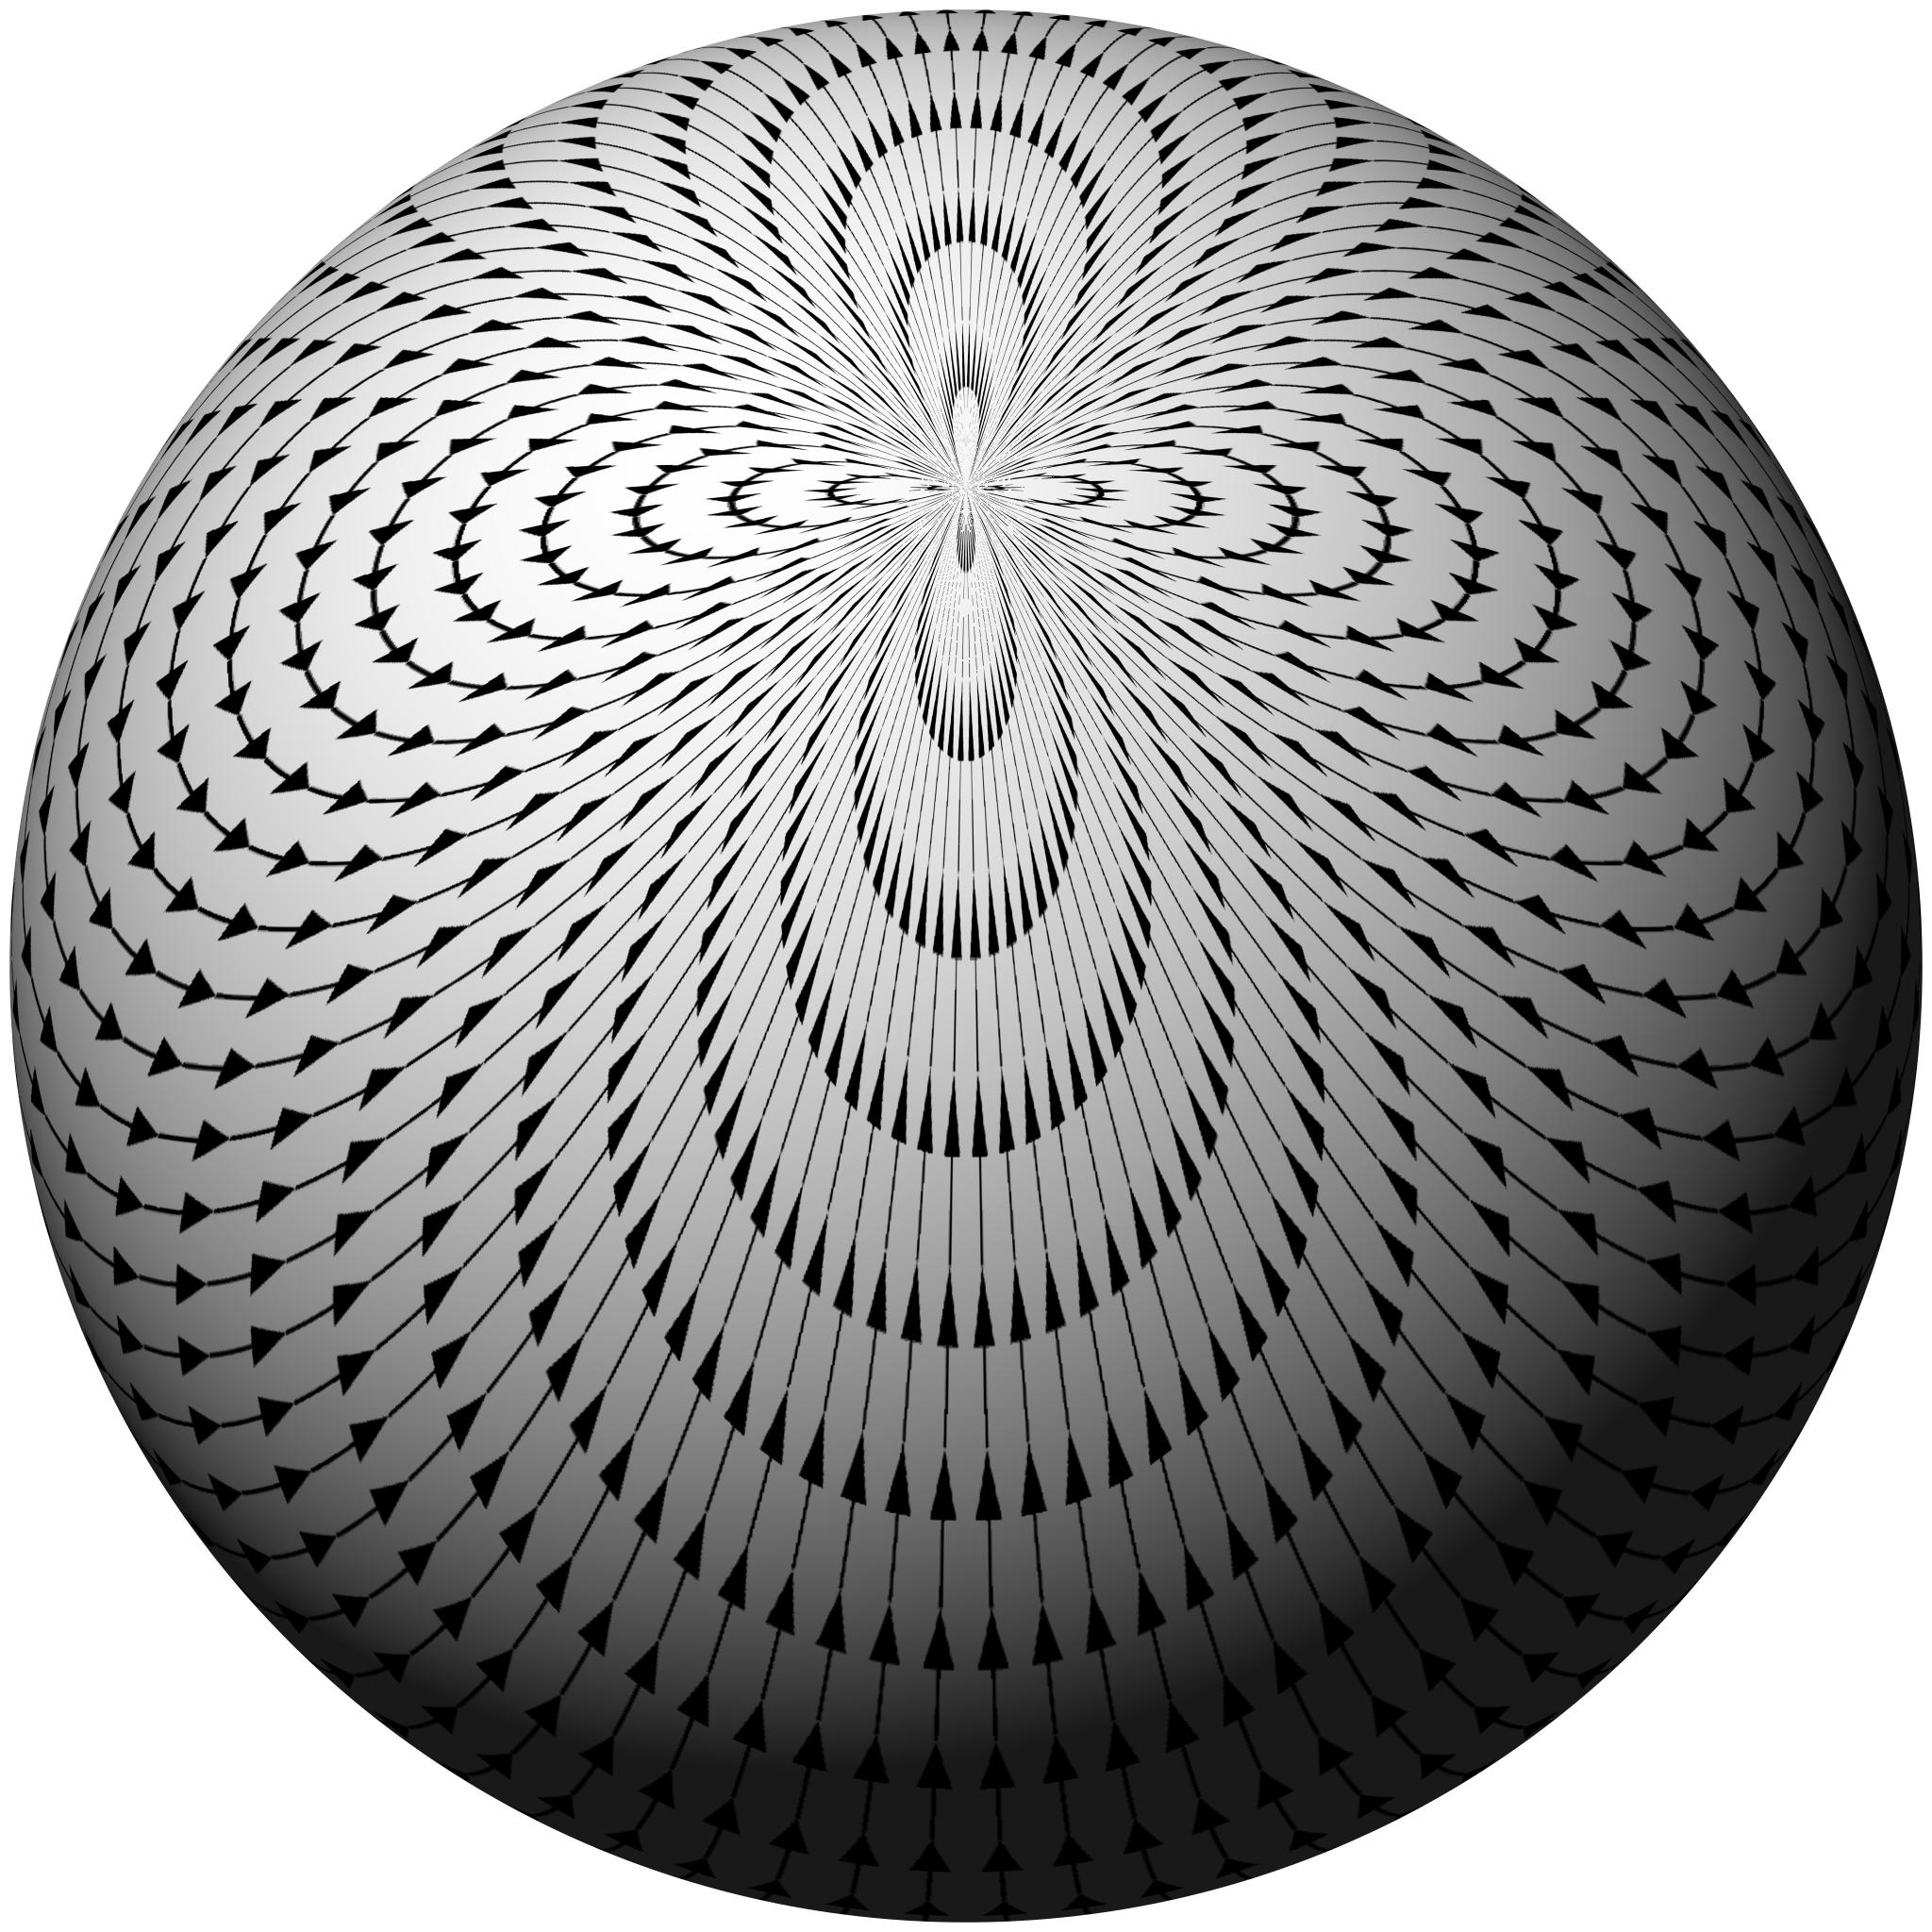
\includegraphics[width=.3\textwidth]{res/Hairy_ball_one_pole}
		   \end{center} 
		   Beim Hertzschen Dipol gibt es (in Fernfeldnäherung) zwei Glatzpunkte, bei $\vartheta=0$ und $\vartheta=\pi$, an denen es kein Feld gibt.
		\subsection{Fitzgeraldscher Dipol}
		    Das zum Hertzschen Dipol \textbf{duale} System ist der \textbf{Fitzgeraldsche Dipol}, eine infinitesimale Leiterschleife mit Flächennormale in \(z\)-Richtung. Es gibt dann  nur \(\ubar{\vec{E}}_\varphi\) und \(\vec{\ubar{H}}_\vartheta\) im Fernfeld. Auch der Fitzgeraldsche Dipol ist ein \textbf{Elementardipol}.
		  
\subsection{Feldwellenimpedanz im Nahfeld der Elementardipole}  
Der Feldwellenwiderstand \(Z=\frac{|\ubar{\vec{E}}|}{|\vec{\ubar{H}}|}\) nur im Fernfeld konstant mit \(Z=120\pi\mathrm{\Omega}\).
\begin{itemize}
	\item[$\to$] Im Nahfeld des Hertzschen Dipols (\ref{dipefeld}$\Rightarrow(kr)^3$, also $E$-Feld dominiert) $\Rightarrow$ \textbf{Hochimpedanzfeld}
	\item[$\to$] Im Nahfeld des Fitzgeraldschen Dipols ($H$-Feld dominiert) $\Rightarrow$ \textbf{Niederimpedanzfeld}
\end{itemize}
Im Nahfeld eines des Hertzschen Dipols ist ein Leiter ein guter Schirm (Außerhalb Hochimpedanzfeld, Leiter niedrige Impedanz $\Rightarrow$ Reflexion groß, $\nearrow$\ref{frenselsref}), im Nahfeld eines Fitzgeraldschen Dipols gilt das nicht. Allgemein gilt, dass elektrisch dominierte Felder einfach zu schirmen sind (einfacher Leiter reicht), während magnetisch dominierte Felder nicht so einfach zu schirmen sind (man braucht sehr teure, hochpermeable Metalle).
  \section{Linearantennen}
  \subsection{Grundlagen}
	 Bei den Elementardipolen (Hertzscher Dipol, Fitzgeraldscher Dipol) gab es infinitesimales Leiterelement und einen zeitlich harmonischen, aber \textbf{räumlich konstanten Strom}. Bei der \textbf{Linearantenne} gibt es einen dünnen, perfekt leitenden Draht, der von einem \textbf{ortsabhängigen} (harmonischen) Wechselstrom \(\underline{I}(\vec{r}^\prime )\) durchflossen wird. \\
	 Zunächst wird nochmal ein Stromelement im Ursprung, also ein Hertzscher Dipol mit etwas anderen Bezeichnungen, betrachtet:
		        \begin{center}
			        % set the plot display orientation
%synatax: \tdplotsetdisplay{\theta_d}{\phi_d}
\tdplotsetmaincoords{60}{110}

%define polar coordinates for some vector
%TODO: look into using 3d spherical coordinate system
\pgfmathsetmacro{\rvec}{.5}
\pgfmathsetmacro{\thetavec}{30}
\pgfmathsetmacro{\phivec}{60}

%start tikz picture, and use the tdplot_main_coords style to implement the display 
%coordinate transformation provided by 3dplot
\begin{tikzpicture}[scale=5,tdplot_main_coords]

	%set up some coordinates 
	%-----------------------
	\coordinate (O) at (0,0,0);

	%determine a coordinate (P) using (r,\theta,\phi) coordinates.  This command
	%also determines (Pxy), (Pxz), and (Pyz): the xy-, xz-, and yz-projections
	%of the point (P).
	%syntax: \tdplotsetcoord{Coordinate name without parentheses}{r}{\theta}{\phi}
	\tdplotsetcoord{P}{\rvec}{\thetavec}{\phivec}

	%draw figure contents
	%--------------------

	%draw the main coordinate system axes
	\draw[thick,->] (0,0,0) -- (.5,0,0) node[anchor=north east]{$x$};
	\draw[thick,->] (0,0,0) -- (0,.5,0) node[anchor=north west]{$y$};
	\draw[thick,->] (0,0,0) -- (0,0,.5) node[anchor=south,pos=0.95]{$z$};

	%draw a vector from origin to point (P) 
	\draw[-stealth,color=red,thick] (O) -- (P) node[midway, below]{$\vec{r} $};
	\draw[-stealth,color=green,thick] (P) -- +(0,0,0.2) node[above]{$\dd \vec{\ubar{A}}=\dd \ubar{A}_z\vu{z}$};

	%draw projection on xy plane, and a connecting line
	\draw[dashed, color=red] (O) -- (Pxy);
	\draw[dashed, color=red] (P) -- (Pxy);

	%draw the angle \phi, and label it
	%syntax: \tdplotdrawarc[coordinate frame, draw options]{center point}{r}{angle}{label options}{label}
	\tdplotdrawarc{(O)}{0.2}{0}{\phivec}{anchor=north}{$\varphi$}

	%set the rotated coordinate system so the x'-y' plane lies within the
	%"theta plane" of the main coordinate system
	%syntax: \tdplotsetthetaplanecoords{\phi}
	\tdplotsetthetaplanecoords{\phivec}

	%draw theta arc and label, using rotated coordinate system
	\tdplotdrawarc[tdplot_rotated_coords]{(0,0,0)}{0.3}{0}{\thetavec}{anchor=south west}{$\vartheta$}

	%draw some dashed arcs, demonstrating direct arc drawing
	%\draw[dashed,tdplot_rotated_coords] (\rvec,0,0) arc (0:90:\rvec);
	%\draw[dashed] (\rvec,0,0) arc (0:90:\rvec);

	%set the rotated coordinate definition within display using a translation
	%coordinate and Euler angles in the "z(\alpha)y(\beta)z(\gamma)" euler rotation convention
	%syntax: \tdplotsetrotatedcoords{\alpha}{\beta}{\gamma}
	\tdplotsetrotatedcoords{\phivec}{\thetavec}{0}

	%translate the rotated coordinate system
	%syntax: \tdplotsetrotatedcoordsorigin{point}
	\tdplotsetrotatedcoordsorigin{(P)}

	%use the tdplot_rotated_coords style to work in the rotated, translated coordinate frame
	%\draw[thin,tdplot_rotated_coords,->] (0,0,0) -- (.1,0,0) node[anchor=north west]{$\vu{\vartheta}$};
	%\draw[thin,tdplot_rotated_coords,->] (0,0,0) -- (0,.1,0) node[anchor=west]{$\vu{\varphi}$};
	%\draw[thin,tdplot_rotated_coords,->] (0,0,0) -- (0,0,.1) node[anchor=south]{$\vu{r}$};

	\node (a) [cylinder, shape border rotate=90, draw, minimum height=5mm, minimum width=2mm,yshift=-1mm] {};
	\draw [<->] ([xshift=-2pt]a.before bottom) -- ([xshift=-2pt]a.after top) node [midway, left] {$\dd z^\prime$};

\end{tikzpicture}
		        \end{center}
		  Für den Beitrag zum Vektorpotential am Punkt \(P\) gilt ($\nearrow$\ref{vekpotdip}):
		        \begin{equation}
			        \dd \vec{\ubar{A}}(\vec{r} ) = \frac{\mu}{4\pi} \underline{I} \dd z^\prime \frac{ \mathrm{e}^{-\mathrm{j} kr}}{r} \vu{z}
		        \end{equation}
		  Für das Magnetfeld folgt ($I$ ist eine Funktion von $r'$, rot wird in Bezug auf $r$ ausgeführt, deshalb nach vorne ziehen mgl.):
		        \begin{equation}\begin{split}
				        \dd\vec{\ubar{H}}(\vec{r} ) &= \frac{1}{\mu} \rot \dd \vec{\ubar{A}}(\vec{r} )\\
				        &= \frac{1}{4\pi} \underline{I} \dd z^\prime \rot \left(\frac{ \mathrm{e}^{-\mathrm{j} kr}}{r} \vu{z}\right)
			        \end{split}\end{equation}
Es wird weiter umgeformt (Nutzung von \ref{rotuv}):
		        \begin{equation}\begin{split}
				        \dd\vec{\ubar{H}}(\vec{r} )  &= \frac{1}{4\pi}\underline{I} \dd z^\prime \rot _{\textcolor{green}{r}}\left(\frac{ \mathrm{e}^{-\mathrm{j} kr}}{r} \vu{z}\right) \\
				        &= \frac{1}{4\pi} \underline{I}\dd z^\prime \bigg[ \frac{ \mathrm{e}^{-\mathrm{j} kr}}{r} \underbrace{\rot \vu{z}}_{=\vec{0}} - \vu{z} \times \textcolor{red}{\grad \left( \frac{ \mathrm{e}^{-\mathrm{j} kr}}{r} \right)}\bigg] \\
				        &= \frac{1}{4\pi} \underline{I}\dd z^\prime \bigg[- \vu{z} \times \textcolor{red}{\left( -\frac{\vec{r} }{r} \left(\frac{1}{r} +\mathrm{j} k \right)   \right) \frac{ \mathrm{e}^{-\mathrm{j} kr}}{r}} \bigg]\\
				        &= \frac{1}{4\pi} \underline{I}\dd z^\prime \left( \vu{z} \times \frac{\vec{r} }{r} \right) \left(\frac{1}{r} +\mathrm{j} k \right) \frac{ \mathrm{e}^{-\mathrm{j} kr}}{r}
			        \end{split}\end{equation}
Für ein Stromelement beliebiger Länge wird der Strom ortsabhängig (\(\underline{I}\to \underline{I}(\vec{r}^\prime )\)). Außerdem können beliebige Leiterelemente und nicht nur $z$-orientierte im Ursprung  betrachtet werden (\(\dd z^\prime \vu{z} \to \dd\vec{r}^\prime \) und \(\vec{r}  \to \vec{r}  - \vec{r}^\prime \)). Das ist unproblematisch (man könnte die ganze Herleitung auch von vornherein so durchziehen). Es gilt damit:
		        \begin{equation}
			        \boxed{\dd\vec{\ubar{H}}(\vec{r} ) = \frac{1}{4\pi} \underline{I}(\vec{r}^\prime ) \left( \dd\vec{r}^\prime  \times \frac{\vec{r} -\vec{r}^\prime }{|\vec{r} -\vec{r}^\prime |} \right) \left(\frac{1}{|\vec{r} -\vec{r}^\prime |} +\mathrm{j} k \right) \frac{ \mathrm{e}^{-\mathrm{j} k |\vec{r} -\vec{r}^\prime |}}{|\vec{r} -\vec{r}^\prime |}}
		        \end{equation}
Im Fernfeld sind folgende Näherungen davon möglich (Näherungen wie in \ref{strahlungszonen}):
		        \begin{equation}\begin{split}
				        k |\vec{r} -\vec{r}^\prime | \gg 1 &\Rightarrow  k \gg \frac{1}{|\vec{r} -\vec{r}^\prime |}\\
				        \frac{\vec{r} -\vec{r}^\prime }{|\vec{r} -\vec{r}^\prime |} &\simeq \frac{\vec{r} }{r}\\
				        \frac{ \mathrm{e}^{-\mathrm{j} k |\vec{r} -\vec{r}^\prime |}}{|\vec{r} -\vec{r}^\prime |} &\simeq \frac{ \mathrm{e}^{-\mathrm{j} k r}}{r}  \mathrm{e}^{\mathrm{j} k \frac{\vec{r} \cdot \vec{r}^\prime }{r}}
			        \end{split}\end{equation}
		  Damit gilt im \textbf{Fernfeld}:
		        \begin{equation}
			        \boxed{\dd\vec{\ubar{H}}(\vec{r} ) = \frac{\mathrm{j} k}{4\pi} \underline{I}(\vec{r}^\prime ) \left( \dd\vec{r}^\prime  \times \frac{\vec{r} }{r} \right) \frac{ \mathrm{e}^{-\mathrm{j} k r}}{r}  \mathrm{e}^{\mathrm{j} k \frac{\vec{r} \cdot \vec{r}^\prime }{r}}}
		        \end{equation}
	  Betrachtet wird nun einen dünner Draht mit Kontur \(C\) als Antenne
		        \begin{center}
			        \begin{tikzpicture}
	{   \colorlet{InColor}{gray!25}
		\colorlet{OutColor}{black!75}
		\foreach \I in {1,...,3}
			{   \pgfmathsetlengthmacro{\h}{(\I-1)/3*2mm}
				\pgfmathsetlengthmacro{\r}{sqrt(pow(2mm,2)-pow(\h,2))}
				\pgfmathsetmacro{\c}{(\I-0.5)/3*100}
				\draw[InColor!\c!OutColor, line width=\r] (0,2) to[out=70,in=200] (5,2);
			}
	}
	\draw (5,2) node[right]{$C$};
	\draw (0,4) node[left]{$0$};
	\draw (6,3.7) node[right]{$P$};
	\draw[-stealth,thick] (0,4) -- (1,2.7) node[midway,left]{$\vec{r}\prime $};
	\draw[-stealth,thick] (0,4) -- (6,3.7) node[midway,below]{$\vec{r} $};
	\draw[-stealth,thick] (1,2.7) -- (6,3.7) node[midway,below]{$\vec{r} -\vec{r}\prime $};
\end{tikzpicture}
		        \end{center}
		  Damit ist das Magnetfeld (und damit auch das elektrische Feld) für beliebige linienförmige Antennen im Fernfeld prinzipiell berechenbar aus:
		        \begin{equation}\label{nhrgfernz}
			        \boxed{\vec{\ubar{H}}(\vec{r} ) = \frac{\mathrm{j} k}{4\pi} \frac{ \mathrm{e}^{-\mathrm{j} k r}}{r} \int\limits_{C}\underline{I}(\vec{r}^\prime )  \mathrm{e}^{\mathrm{j} k \frac{\vec{r} \cdot \vec{r}^\prime }{r}} \left( \dd\vec{r}^\prime  \times \frac{\vec{r} }{r} \right)}
		        \end{equation}
		        Analog kann man im \textbf{Nahfeld} die Retardierung vernachlässigen und magnetoquasistatisch Biot-Savart ansetzen. Man sollte sich dabei aber stets vergegenwärtigen, welche Annahmen in den genutzten Formeln stecken und prüfen ob diese (näherungsweise) haltbar sind. Dadurch wird verhindert, dass schlechte Näherungen entstehen.
	\subsection{Beispiel}
	\subsubsection{Problemstellung}
	Eine halbkreisförmige Antenne aus sehr dünnem idealleitendem ($\kappa\to\infty$) Drat befindet sich im Vakuum. Drei Punkte auf der Antenne können kartesisch als $P_1(0,-a,0)$, $P_2(0,a,0)$ und $P_3(-a,0,0)$ beschrieben werden. Die Antenne führt einen harmonischen Wechselstrom $\vec{\ubar{I}}(\vec{r})=I_0\vu{\varphi}$. Dafür muss $a\ll\lambda$ gelten, sonst könnte der Strom nicht auf der gesamten Antenne als räumlich konstant angenommen werden (exakt müsste der Strom durch eine auf dem Antennendraht propagierende Welle beschrieben werden).
	\begin{center}
			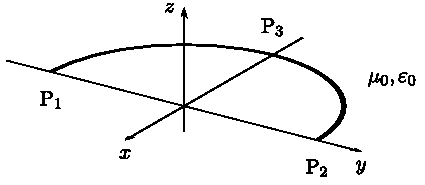
\includegraphics{res/ANTbsp.pdf}
	\end{center}
		\subsubsection{Exakte Berechnung von Vektorpotential und Magnetfeld auf der z-Achse}
	Zunächst sollen $\vec{{A}}(z,t)$ und $\vec{H}(z,t)$ auf der $z$-Achse exakt berechnet werden. Für $\vec{A}(z,t)$ wird die allgemeine Gleichung \ref{vekpotlor} angesetzt. Es gilt:
	\begin{equation}
		\vec{{A}}(z, {t})=\frac{\mu_{0}}{4 \pi} \iiint\limits_V \frac{\vec{{J}}\left(\vec{{r}}^{\prime}, {t}_{\text{ret}}\right)}{\left|z\vu{z}-\vec{{r}}^{\prime}\right|} \dd^3 {r}^{\prime} \quad \text{ mit } \quad t_{\text{ret}}={t}-\frac{\left|z\vu{z}-\vec{{r}}^{\prime}\right|}{{c}}
	\end{equation}
	Zunächst muss $\vec{{J}}\left(\vec{{r}}^{\prime}, {t}\right)$ modelliert werden:
	\begin{equation}
		\vec{{J}}\left(\vec{{r}}^{\prime}, {t}\right)=I_{0} \cos\left(\omega t\right)\delta\left(\rho'-a \right) \delta\left(z' \right)\vu{\varphi} (\varphi')
	\end{equation}
	Einsetzen liefert:
	\begin{equation}
		\vec{{A}}(z, {t})=\frac{\mu_{0}}{4 \pi} \iiint\limits_V \frac{I_{0} \cos\left[\omega\left( {t}-\frac{\left|z\vu{z}-\vec{{r}}^{\prime}\right|}{{c}}\right)\right]\delta\left(\rho'-a \right) \delta\left(z' \right)\vu{\varphi}(\varphi') }{\left|z\vu{z}-\vec{{r}}^{\prime}\right|} \rho'\dd\rho'\dd\varphi'\dd z' 
	\end{equation}
	Integration über das Quellgebiet (Halbraum mit $x\leq0$, man könnte auch über den gesamten Raum integrieren und noch mit $J$ noch zusätzlich mit einer Stufenfunktion modellieren) liefert:
	\begin{equation}\begin{split}
			\vec{{A}}(z, {t})&=\frac{\mu_{0}I_{0} a}{4 \pi} \frac{\cos\left[\omega \left({t}-\frac{\sqrt{z^2+a^2}}{{c}}\right)\right] }{\sqrt{a^2+z^2}}\int\limits_{\varphi'=\frac{\pi}{2}}^{\frac{3\pi}{2}} \vu{\varphi}(\varphi')\dd \varphi'\\
			&=-\vu{y}\frac{\mu_{0}I_{0} a}{2 \pi} \frac{\cos\left[\omega \left({t}-\frac{\sqrt{z^2+a^2}}{{c}}\right)\right] }{\sqrt{a^2+z^2}}
	\end{split}\end{equation}
\textbf{Fehlerquelle:} Würde man nun mit diesem Ergebnis weiterrechnen, und versuchen über $\vec{H}=\frac{1}{\mu_0}\rot\vec{A}$ das Magnetfeld herzuleiten, würde man auf ein falsches Ergebnis kommen. Das liegt daran, dass in die Rotation auch die Ableitungen nach $x$ und $y$ eingehen, welche trotz $x=y=0$ nicht zwangsläufig null sind, aber durch Betrachtung von $\vec{{A}}(z, {t})$ statt $\vec{{A}}(\vec{r}, {t})$ null gesetzt werden würden. Es gilt also:
\begin{equation}
	\vec{H}(z, {t})=\left.\frac{1}{\mu_0}\rot\vec{A}(\vec{r}, {t}) \right|_{x=y=0}\neq \frac{1}{\mu_0}\rot\vec{A}(z, {t})
\end{equation}
Demnach muss $\vec{H}(z, {t})$ ausführlich berechnet werden:
\begin{equation}
		\vec{{H}}(z, {t})=\left.\frac{I_{0} a}{4 \pi} \int\limits_{\varphi'=\frac{\pi}{2}}^{\frac{3\pi}{2}} \rot_r\frac{\cos\left[\omega \left({t}-\frac{\left|\rho\vu{\rho}(\varphi)-a\vu{\rho}(\varphi')+z\vu{z}\right|}{{c}}\right)\right] }{\left|\rho\vu{\rho}(\varphi)-a\vu{\rho}(\varphi')+z\vu{z}\right|} \vu{\varphi}(\varphi')\dd \varphi'\right|_{\rho=0}
\end{equation}
\textbf{Fehlerquelle:} Die Rotation im Integral ist bezüglich $r$ und nicht $r'$ zu berechnen. Es ist demnach bei der Rotationsbildung zu beachten, dass die $\vu{\varphi}(\varphi')$-Komponente bezüglich der gestrichenen Koordinaten eine $\vu{\varphi}(\varphi)$- \textbf{und} eine $\vu{\rho}(\varphi)$-Komponente bezüglich der ungestrichenen Koordinaten bedeutet. Nun soll die Rotation berechnet werden, um das Problem mit der $\vu{\varphi}(\varphi')$-Komponente zielgerichtet zu umgehen, bietet sich eine zweimalige Anwendung der Produktregel \ref{rotuv} an:
\begin{equation*}\begin{split}
	&\rot_r\underbrace{\frac{1}{\left|\rho\vu{\rho}(\varphi)-a\vu{\rho}(\varphi')+z\vu{z}\right|}}_{U} \underbrace{\cos\left[\omega \left({t}-\frac{\left|\rho\vu{\rho}(\varphi)-a\vu{\rho}(\varphi')+z\vu{z}\right|}{{c}}\right)\right]  \vu{\varphi}(\varphi')}_{\vec{V}}\\
	&\quad=\frac{1}{\left|\rho\vu{\rho}(\varphi)-a\vu{\rho}(\varphi')+z\vu{z}\right|}\rot_r\left\{\underbrace{\cos\left[\omega \left({t}-\frac{\left|\rho\vu{\rho}(\varphi)-a+z\vu{z}\right|}{{c}}\right)\right]}_{U} \underbrace{\vu{\varphi}(\varphi')}_{\vec{V}}  \right\} \\
	&\quad\quad+ \grad_r\left\{\frac{1}{\left|\rho\vu{\rho}(\varphi)-a\vu{\rho}(\varphi')+z\vu{z}\right|}\right\}\times\cos\left[\omega \left({t}-\frac{\left|\rho\vu{\rho}(\varphi)-a\vu{\rho}(\varphi')+z\vu{z}\right|}{{c}}\right)\right]  \vu{\varphi}(\varphi')\\
	&\quad=\frac{1}{\left|\rho\vu{\rho}(\varphi)-a\vu{\rho}(\varphi')+z\vu{z}\right|}\left( \underbrace{0}_{\vu{\varphi}(\varphi')\neq f(\vec{r})}+ \grad_r\left\{\cos\left[\omega \left({t}-\frac{\left|\rho\vu{\rho}(\varphi)-a+z\vu{z}\right|}{{c}}\right)\right]\right\}\times\vu{\varphi}(\varphi') \right)\\
	&\quad\quad+ \grad_r\left\{\frac{1}{\left|\rho\vu{\rho}(\varphi)-a\vu{\rho}(\varphi')+z\vu{z}\right|}\right\}\times\cos\left[\omega \left({t}-\frac{\left|\rho\vu{\rho}(\varphi)-a\vu{\rho}(\varphi')+z\vu{z}\right|}{{c}}\right)\right]  \vu{\varphi}(\varphi')
\end{split}\end{equation*}
\textbf{Fehlerquelle:} Im Allgemeinen ist $\vu{\rho}(\varphi)\neq\vu{\rho}(\varphi')$, die Betragsbildung muss über den Cosinussatz in der $z=0$-Ebene oder die Identität $\vu{\rho}(\varphi)=\vu{x}\cos\varphi+\vu{y}\sin\varphi$ erfolgen. Mit dem Cosinussatz gilt:
\begin{equation*}
	\left|\rho\vu{\rho}(\varphi)-a\vu{\rho}(\varphi')+z\vu{z}\right|=\sqrt{\rho^2+a^2-2\rho a\cos{\left(\varphi-\varphi'\right)}+z^2}
\end{equation*}
Damit ist
\begin{equation*}\begin{split}
	&\left.\grad_r\left\{\frac{1}{\sqrt{\rho^2+a^2-2\rho a\cos{\left(\varphi-\varphi'\right)}+z^2}}\right\}\right|_{\rho=0}=\\
	&\quad+\vu{\rho}(\varphi)\frac{a\cos{\left(\varphi-\varphi'\right)}}{(a^2+z^2)^{\frac{3}{2}}} -\vu{\varphi}(\varphi)\frac{a \sin{\left(\varphi-\varphi'\right)}}{(a^2+z^2)^{\frac{3}{2}}} -\vu{z}\frac{z}{(a^2+z^2)^{\frac{3}{2}}}\\
	&\quad:=\vu{\rho}(\varphi)A\cos{\left(\varphi-\varphi'\right)}-\vu{\varphi}(\varphi)A\sin{\left(\varphi-\varphi'\right)}+\vu{z}B\\
	&\left.\grad_r\left\{\cos\left[\omega \left({t}-\frac{\sqrt{\rho^2+a^2-2\rho a\cos{\left(\varphi-\varphi'\right)}+z^2}}{{c}}\right)\right]\right\}\right|_{\rho=0}=\\
	&\quad-\vu{\rho}(\varphi)\frac{a\omega\cos{\left(\varphi-\varphi'\right)}\sin\left[\omega \left({t}-\frac{\sqrt{a^2+z^2}}{{c}}\right)\right]}{c\sqrt{a^2+z^2}}+\vu{\varphi}(\varphi)\frac{a\omega\sin{\left(\varphi-\varphi'\right)}\sin\left[\omega \left({t}-\frac{\sqrt{a^2+z^2}}{{c}}\right)\right]}{c\sqrt{a^2+z^2}}\\
	&\quad+\vu{z}\frac{\omega z\sin\left[\omega \left({t}-\frac{\sqrt{a^2+z^2}}{{c}}\right)\right]}{c\sqrt{a^2+z^2}}:=\vu{\rho}(\varphi)C\cos{\left(\varphi-\varphi'\right)}-\vu{\varphi}(\varphi)C\sin{\left(\varphi-\varphi'\right)}+\vu{z}D
\end{split}\end{equation*}
Damit und mit den Definitionen
\begin{equation*}\begin{split}
 E:=&\frac{1}{\sqrt{z^2+a^2}}\\
 F:=&\cos\left[\omega \left({t}-\frac{\sqrt{a^2+z^2}}{{c}}\right)\right]
\end{split}\end{equation*}
folgt ($k=\frac{\omega}{c}$):
\begin{equation*}\begin{split}
		\vec{{H}}(z, {t})&=\frac{I_{0} a}{4 \pi}\int\limits_{\varphi'=\frac{\pi}{2}}^{\frac{3\pi}{2}} E\left[\vu{\rho}(\varphi)C\cos{\left(\varphi-\varphi'\right)}+\vu{\varphi}(\varphi)-C\sin{\left(\varphi-\varphi'\right)}+\vu{z}D\right]\times\left[\vu{\varphi}(\varphi')\right]\\\quad&+F\left[\vu{\rho}(\varphi)A\cos{\left(\varphi-\varphi'\right)}-\vu{\varphi}(\varphi)A\sin{\left(\varphi-\varphi'\right)}+\vu{z}B\right]\times\left[\vu{\varphi}(\varphi')\right] \dd \varphi'
	\end{split}\end{equation*}
Dieses Integral kann man unter Nutzung der Identitäten
\begin{equation*}
	\begin{split}
	\vu{\varphi}(\varphi)&=-\vu{x}\sin\varphi+\vu{y}\cos\varphi\\
	\vu{\rho}(\varphi)&=\vu{x}\cos\varphi+\vu{y}\sin\varphi	
	\end{split}
\end{equation*}
ausrechnen und erhält:
\begin{equation}\label{hallgbsp}\begin{split}
		\vec{{H}}(z, {t})&=\frac{I_{0} a}{4 \pi}\left[E\left(\vu{z}\pi C+\vu{x}2D\right)+F\left(\vu{z}\pi A+\vu{x}2B\right)\right]\\
		&=\frac{I_{0} a}{4 \pi}(-a\pi\vu{z}+2z\vu{x})\left[\frac{k\sin\left[\omega {t}-k\sqrt{z^2+a^2}\right]}{z^2+a^2}-\frac{\cos\left[\omega {t}-k\sqrt{z^2+a^2}\right]}{\left(z^2+a^2\right)^{\frac{3}{2}}}\right]
\end{split}\end{equation}
\subsubsection{Nahzone}
In der Nahzone gilt nach \ref{strahlungszonen} $a\ll |z|\ll\lambda$. Mit $k=\frac{2\pi}{\lambda}$ kann man \ref{hallgbsp} nähern:
\begin{equation}\label{hallgbspapprox}\begin{split}
	\vec{{H}}(z, {t})=-\frac{I_{0} a}{2 \pi}\underbrace{z\vu{x}}_{z\gg a}\underbrace{\frac{\cos\left[\omega {t}\right]}{\left(z^2+a^2\right)^{\frac{3}{2}}}}_{\lambda\gg z \gg a}
\end{split}\end{equation}
Mit Biot-Savart ($\nearrow$\ref{biot-savart}) kommt man auf:
\begin{equation}
	\vec{{H}}(z, {t})=\frac{I_{0} a}{4 \pi}(a\pi\vu{z}-2z\vu{x})\frac{\cos\left[\omega {t}\right]}{\left(z^2+a^2\right)^{\frac{3}{2}}}
\end{equation}
Offensichtlich fehlt hier gegenüber \ref{hallgbsp} die Retardierung (quasistatische Näherung) und einer der beiden Terme in der eckigen Klammer. Nach anwenden von $z\gg a$ kommt man auf die selbe Näherungsformel wie in \ref{hallgbspapprox}. In der Nahzone erhält man hier also mit Biot-Savart eine brauchbare Näherung.
\subsubsection{Fernzone}
In der Fernzone gilt nach \ref{strahlungszonen} $a\ll |z|$ und $\lambda\ll |z|$. Mit $k=\frac{2\pi}{\lambda}$ kann man \ref{hallgbsp} wieder nähern:
\begin{equation}
	\begin{split}
		\vec{{H}}(z, {t})=\vu{x} \frac{I_{0} a}{2 \pi}\frac{k\sin\left[\omega {t}-k|z|\right]}{z}
	\end{split}
\end{equation}
Mit der Näherungsformel für die Fernzone aus Gleichung \ref{nhrgfernz} kommt man auf exakt das gleiche Ergebnis.
  \subsection{Abstrahldiagramme und Bauformen}
  $n\lambda$-Dipol meint, dass man auf die gesamte Drahtstruktur genau $n$ mal die Wellenlänge bekommt. Die Speisung der Antennenstruktur ist mit einem Pfeil gekennzeichnet. Gewünscht ist meist eine gerichtete Abstrahlung, technisch bewegt man sich also häufig im Bereich des $\frac{\lambda}{2}$-Dipols. Beim $\frac{\lambda}{4}$-Dipol ersetzt man die untere Leitung vom $\frac{\lambda}{2}$-Dipol durch eine leidende Ebene, durch das Spiegelungsprinzip ist das Feld dann ähnlich wie beim $\frac{\lambda}{2}$-Dipol. Durch dielektrische Materialien, Fußinduktivitäten und Dachkapazitäten kann man elektrisch eine längere Antenne erreichen, als tatsächlich physikalisch vorliegt (bspw. Antenne nur $\frac{\lambda}{8}$ groß, aber elektrisch wirksam als $\frac{\lambda}{2}$). Anschauung (\href{https://commons.wikimedia.org/wiki/File:Lineare_antennen2.svg}{Bildquelle}):,
	  \begin{center}
		  \resizebox{.6\textwidth}{!}{%% Creator: Inkscape 1.3 (1:1.3+202307231459+0e150ed6c4), www.inkscape.org
%% PDF/EPS/PS + LaTeX output extension by Johan Engelen, 2010
%% Accompanies image file 'Lineare_antennen2.pdf' (pdf, eps, ps)
%%
%% To include the image in your LaTeX document, write
%%   \input{<filename>.pdf_tex}
%%  instead of
%%   \includegraphics{<filename>.pdf}
%% To scale the image, write
%%   \def\svgwidth{<desired width>}
%%   \input{<filename>.pdf_tex}
%%  instead of
%%   \includegraphics[width=<desired width>]{<filename>.pdf}
%%
%% Images with a different path to the parent latex file can
%% be accessed with the `import' package (which may need to be
%% installed) using
%%   \usepackage{import}
%% in the preamble, and then including the image with
%%   \import{<path to file>}{<filename>.pdf_tex}
%% Alternatively, one can specify
%%   \graphicspath{{<path to file>/}}
%% 
%% For more information, please see info/svg-inkscape on CTAN:
%%   http://tug.ctan.org/tex-archive/info/svg-inkscape
%%
\begingroup%
\makeatletter%
\providecommand\color[2][]{%
	\errmessage{(Inkscape) Color is used for the text in Inkscape, but the package 'color.sty' is not loaded}%
	\renewcommand\color[2][]{}%
}%
\providecommand\transparent[1]{%
	\errmessage{(Inkscape) Transparency is used (non-zero) for the text in Inkscape, but the package 'transparent.sty' is not loaded}%
	\renewcommand\transparent[1]{}%
}%
\providecommand\rotatebox[2]{#2}%
\newcommand*\fsize{\dimexpr\f@size pt\relax}%
\newcommand*\lineheight[1]{\fontsize{\fsize}{#1\fsize}\selectfont}%
\ifx\svgwidth\undefined%
	\setlength{\unitlength}{363.32178497bp}%
	\ifx\svgscale\undefined%
		\relax%
	\else%
		\setlength{\unitlength}{\unitlength * \real{\svgscale}}%
	\fi%
\else%
	\setlength{\unitlength}{\svgwidth}%
\fi%
\global\let\svgwidth\undefined%
\global\let\svgscale\undefined%
\makeatother%
\begin{picture}(1,1.16380096)%
	\lineheight{1}%
	\setlength\tabcolsep{0pt}%
	\put(0,0){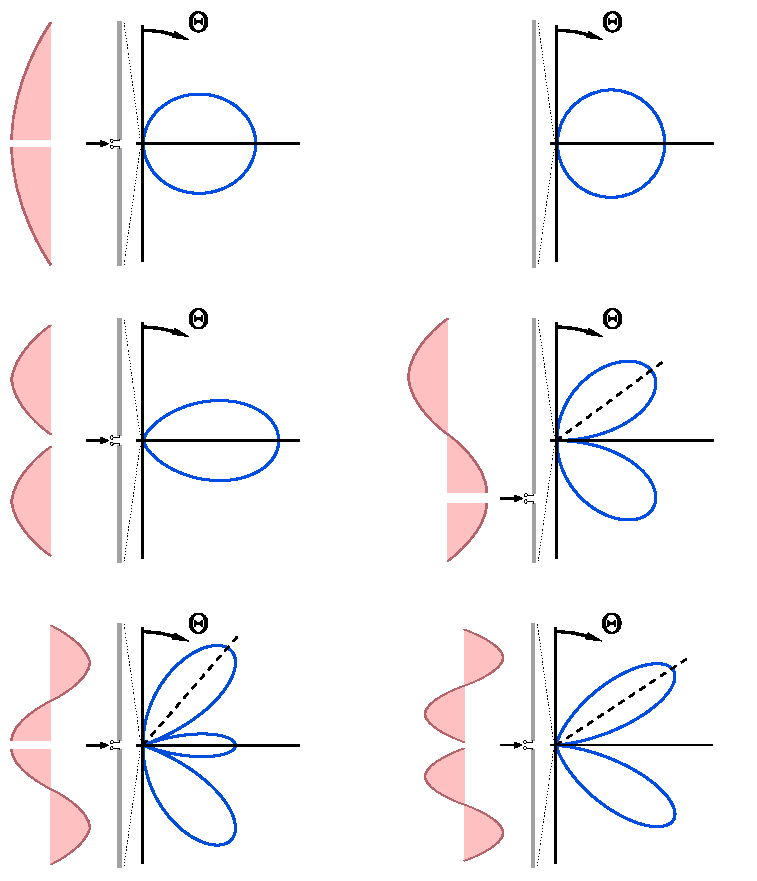
\includegraphics[width=\unitlength,page=1]{res/Lineare_antennen2.pdf}}%
	\put(-0.03749462,1.13927431){\color[rgb]{0,0,0}\makebox(0,0)[lt]{\lineheight{1.25}\smash{\begin{tabular}[t]{l}\textbf{Stomverteilung}\end{tabular}}}}%
	\put(0.21682177,1.05874075){\color[rgb]{0,0,0}\makebox(0,0)[lt]{\lineheight{1.25}\smash{\begin{tabular}[t]{l}\textbf{Fernfeld}\end{tabular}}}}%
	\put(0,0){\includegraphics[width=\unitlength,page=2]{res/Lineare_antennen2.pdf}}%
	\put(0.25016422,1.12146949){\color[rgb]{0,0,0}\makebox(0,0)[lt]{\lineheight{1.25}\smash{\begin{tabular}[t]{l}$\vartheta$\end{tabular}}}}%
	\put(0.24944189,0.72793128){\color[rgb]{0,0,0}\makebox(0,0)[lt]{\lineheight{1.25}\smash{\begin{tabular}[t]{l}$\vartheta$\end{tabular}}}}%
	\put(0.24899603,0.32657848){\color[rgb]{0,0,0}\makebox(0,0)[lt]{\lineheight{1.25}\smash{\begin{tabular}[t]{l}$\vartheta \quad 43^\circ$ \end{tabular}}}}%
	\put(0.79733669,1.12329457){\color[rgb]{0,0,0}\makebox(0,0)[lt]{\lineheight{1.25}\smash{\begin{tabular}[t]{l}$\vartheta$\end{tabular}}}}%
	\put(0.79595453,0.72835632){\color[rgb]{0,0,0}\makebox(0,0)[lt]{\lineheight{1.25}\smash{\begin{tabular}[t]{l}$\vartheta$\\$\quad\quad 54^\circ$\end{tabular}}}}%
	\put(0.78974511,0.32540434){\color[rgb]{0,0,0}\makebox(0,0)[lt]{\lineheight{1.25}\smash{\begin{tabular}[t]{l}$\vartheta$\\$\quad\quad\quad\quad 57^\circ$\\\end{tabular}}}}%
	\put(0.19493004,0.81773808){\color[rgb]{0,0,0}\makebox(0,0)[lt]{\lineheight{1.25}\smash{\begin{tabular}[t]{l}$\frac{\lambda}{2}$-Dipol\end{tabular}}}}%
	\put(0.19305147,0.42551962){\color[rgb]{0,0,0}\makebox(0,0)[lt]{\lineheight{1.25}\smash{\begin{tabular}[t]{l}$\lambda$-Dipol\end{tabular}}}}%
	\put(0.19487356,0.02299265){\color[rgb]{0,0,0}\makebox(0,0)[lt]{\lineheight{1.25}\smash{\begin{tabular}[t]{l}$\frac{3\lambda}{2}$-Dipol\end{tabular}}}}%
	\put(0.7386129,0.02186903){\color[rgb]{0,0,0}\makebox(0,0)[lt]{\lineheight{1.25}\smash{\begin{tabular}[t]{l}$2\lambda$-Dipol\end{tabular}}}}%
	\put(0.73937976,0.42576928){\color[rgb]{0,0,0}\makebox(0,0)[lt]{\lineheight{1.25}\smash{\begin{tabular}[t]{l}$\lambda$-Dipol\\(asymmetrische Sp.)\end{tabular}}}}%
	\put(0.73798866,0.81912619){\color[rgb]{0,0,0}\makebox(0,0)[lt]{\lineheight{1.25}\smash{\begin{tabular}[t]{l}Hertzscher Dipol\end{tabular}}}}%
	\put(0,0){\includegraphics[width=\unitlength,page=3]{res/Lineare_antennen2.pdf}}%
\end{picture}%
\endgroup%
}
		  	  \end{center}
		  	  Halbwellendipole werden häufig zu Kalibrierzwecken eingesetzt, sie sind aber nicht sehr breitbandig, man benötigt verschiedene / verstellbare Bauformen. Breitbandiger sind beispielsweise logarithmisch-periodische Antennen. Bei verschiedenen Frequenzen schwingen verschiedene Stabpaare. Für die Abstrahlungen von Pulsen sind sie aber nicht geeignet. Bikonische Antennen sind ein Beispiel von Dachkapazitäten, man kann also mit kürzerer physikalischer Antenne die gewünschte Wellenlänge erreichen. Außerdem sorgt die Bauform für eine gewisse Breitbandigkeit. Bikoni-Log-Antennen sind Mischformen zwischen logarithmischen und bikonischen Antennen. Die Loop-Antenne ist eine magnetische Antenne, die ein Niederimpedanzfeld im Nahfeld erzeugt. Der eigentliche Draht läuft innen drin, außen gibt es einen massiven (geschlitzten) Zylinder, der die Antenne vor dem elektrischen Feld schützt, wenn nur das Magnetfeld gemessen werden soll. Die Bilder stammen von der Firma \href{https://www.schwarzbeck.de/}{Schwarzbeck}.
		  	  \begin{center}
		  \resizebox{.6\textwidth}{!}{%% Creator: Inkscape 1.3 (1:1.3+202307231459+0e150ed6c4), www.inkscape.org
%% PDF/EPS/PS + LaTeX output extension by Johan Engelen, 2010
%% Accompanies image file 'Antennen-Bilder.pdf' (pdf, eps, ps)
%%
%% To include the image in your LaTeX document, write
%%   \input{<filename>.pdf_tex}
%%  instead of
%%   \includegraphics{<filename>.pdf}
%% To scale the image, write
%%   \def\svgwidth{<desired width>}
%%   \input{<filename>.pdf_tex}
%%  instead of
%%   \includegraphics[width=<desired width>]{<filename>.pdf}
%%
%% Images with a different path to the parent latex file can
%% be accessed with the `import' package (which may need to be
%% installed) using
%%   \usepackage{import}
%% in the preamble, and then including the image with
%%   \import{<path to file>}{<filename>.pdf_tex}
%% Alternatively, one can specify
%%   \graphicspath{{<path to file>/}}
%% 
%% For more information, please see info/svg-inkscape on CTAN:
%%   http://tug.ctan.org/tex-archive/info/svg-inkscape
%%
\begingroup%
\makeatletter%
\providecommand\color[2][]{%
	\errmessage{(Inkscape) Color is used for the text in Inkscape, but the package 'color.sty' is not loaded}%
	\renewcommand\color[2][]{}%
}%
\providecommand\transparent[1]{%
	\errmessage{(Inkscape) Transparency is used (non-zero) for the text in Inkscape, but the package 'transparent.sty' is not loaded}%
	\renewcommand\transparent[1]{}%
}%
\providecommand\rotatebox[2]{#2}%
\newcommand*\fsize{\dimexpr\f@size pt\relax}%
\newcommand*\lineheight[1]{\fontsize{\fsize}{#1\fsize}\selectfont}%
\ifx\svgwidth\undefined%
	\setlength{\unitlength}{755.85667419bp}%
	\ifx\svgscale\undefined%
		\relax%
	\else%
		\setlength{\unitlength}{\unitlength * \real{\svgscale}}%
	\fi%
\else%
	\setlength{\unitlength}{\svgwidth}%
\fi%
\global\let\svgwidth\undefined%
\global\let\svgscale\undefined%
\makeatother%
\begin{picture}(1,0.33178116)%
	\lineheight{1}%
	\setlength\tabcolsep{0pt}%
	\put(0,0){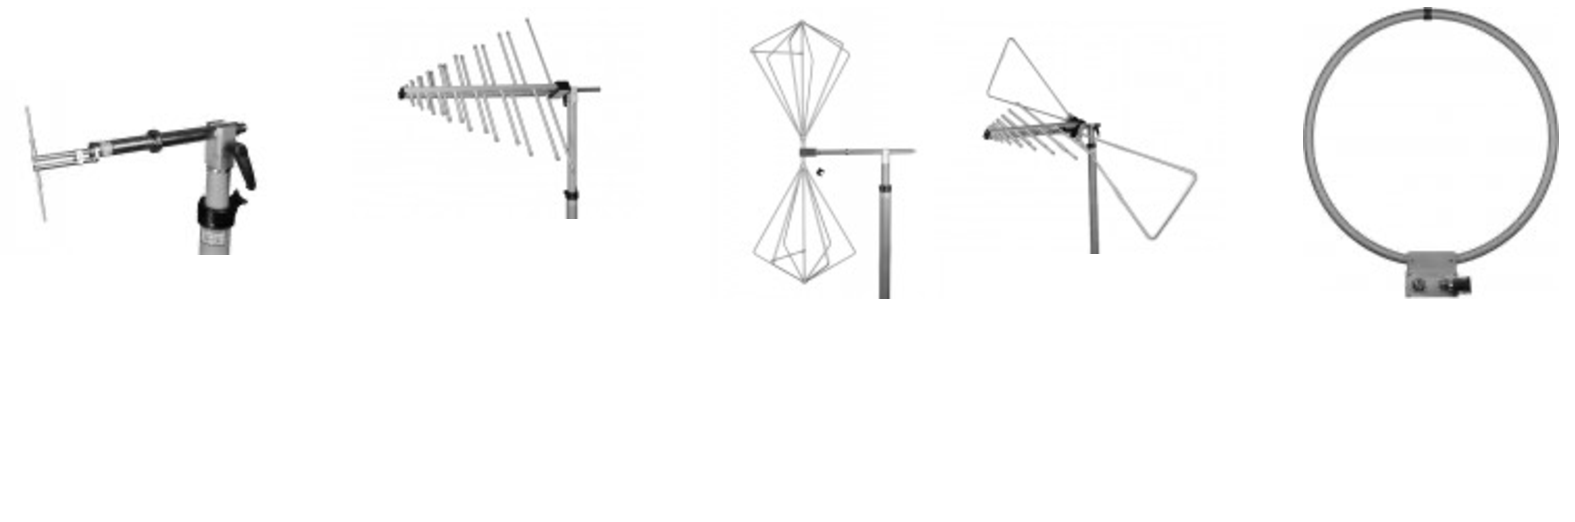
\includegraphics[width=\unitlength,page=1]{res/Antennen-Bilder.pdf}}%
	\put(0.02529879,0.1033566){\color[rgb]{0,0,0}\makebox(0,0)[lt]{\lineheight{1.25}\smash{\begin{tabular}[t]{l}\huge Halbwellendipol\end{tabular}}}}%
	\put(0.25964113,0.1033566){\color[rgb]{0,0,0}\makebox(0,0)[lt]{\lineheight{1.25}\smash{\begin{tabular}[t]{l}\huge Logarithmisch-\\\huge Periodische\\ \huge Antenne\end{tabular}}}}%
	\put(0.48558592,0.1033566){\color[rgb]{0,0,0}\makebox(0,0)[lt]{\lineheight{1.25}\smash{\begin{tabular}[t]{l}\huge Bikonische\\ \huge Antenne\end{tabular}}}}%
	\put(0.65109789,0.1033566){\color[rgb]{0,0,0}\makebox(0,0)[lt]{\lineheight{1.25}\smash{\begin{tabular}[t]{l}\huge Bikoni-Log-\\\huge Antenne\end{tabular}}}}%
	\put(0.83275261,0.10400776){\color[rgb]{0,0,0}\makebox(0,0)[lt]{\lineheight{1.25}\smash{\begin{tabular}[t]{l}\huge Loop-Antenne\\\huge (geschirmt)\end{tabular}}}}%
\end{picture}%
\endgroup%
}
	  \end{center}

